%\documentclass[hidelinks]{report}
%\usepackage[english]{babel}
\usepackage{illcmolthesis}
\usepackage{microtype}
\usepackage{amsmath,amssymb}
\usepackage{amsthm}
\usepackage[round, authoryear]{natbib}
\usepackage[all]{xy}
\usepackage{array}
\usepackage{graphicx}
\usepackage{framed}
\usepackage{enumerate}
\usepackage{qtree}
\usepackage{mdframed}
\usepackage{tikz}
\usepackage{multirow}
\usepackage{pgfplots}
\pgfplotsset{compat = newest}
\usepackage{tikz-dependency}
\usepackage{xfrac}
\usepackage{algorithmic}
\usepackage{algorithm}
\usepackage{float}
\usepackage[OT2,T1]{fontenc}
\usepackage{hyperref}
\newcommand\textcyr[1]{{\fontencoding{OT2}\fontfamily{wncyr}\selectfont #1}}
\newcommand{\myparagraph}[1]{\paragraph{#1}\mbox{}\\}
\bibliographystyle{plainnat}
\renewcommand\topfraction{0.85}
\renewcommand\bottomfraction{0.85}
\renewcommand\textfraction{0.1}
\renewcommand\floatpagefraction{0.85}

%Define theorem style for definition and metric
\newtheoremstyle{break}  % follow `plain` defaults but change HEADSPACE.
  {\topsep}   % ABOVESPACE
  {15pt}   % BELOWSPACE
  {\itshape}  % BODYFONT
  {0pt}       % INDENT (empty value is the same as 0pt)
  {\bfseries} % HEADFONT
  {.}         % HEADPUNCT
  {\newline}  % HEADSPACE. `plain` default: {5pt plus 1pt minus 1pt}
  {}          % CUSTOM-HEAD-SPEC

\theoremstyle{break}
\newtheorem{metric}{Metric}
\newtheorem{notion}{Notion}
\newtheorem{definition}{Definition}
\def\citepos#1{\citeauthor{#1}'s (\citeyear{#1})}

%Define new float environment for tables that is boxed
\floatstyle{boxed}
\newfloat{tab}{tbp}{lop}
\floatname{tab}{Table}
%\begin{document}

\chapter{An Empirical Account of Compositionality}

In the previous chapters, we sketched the background for this thesis, introduced the translation strategy we are investigating, and argued that further research to this strategy is necessary. In the rest of this thesis, we will discuss the research that we have conducted that contributes to this topic. The remainder of this thesis is divided in three parts. In the current chapter, we will discuss the foundations of our study. We will formulate our research questions, discuss the assumptions that we make in investigating them, and discuss the design choices that are made regarding the basic ingredients of our experiments. In the subsequent chapter (Chapter \ref{chap:exp}) the empirical answers that we have found regarding the correspondence between dependency parses and alignment trees will be presented, as well as details about the experiments designed to obtain these results. Finally, in Chapter 6, we will provide a more general discussion of our work, propose an approach to overcome the difficulties that we have found in the experiments, and make suggestions for future work.

We will start this chapter by clearly stating what the main goals of this thesis are. This will include a recap of the motivation for this research. We will formulate the research questions that will be addressed, and of what nature the answers will be (Section \ref{sec:goals}). This section will end with a short remark on compositionality, and its empirical interpretation. In the subsequent section (Section \ref{sec:setup}), we will present the general set-up, and inform the reader about the proceedings of the rest of the chapter, in which the different ingredients of our research are discussed in more detail (Section \ref{sec:assumptions} - \ref{sec:comp_structures2}). Once again, the Chapter finishes with a brief summary.


\section{Summary and Objectives}
\label{sec:goals}

This thesis addresses the appropriateness of compositional translation as a strategy for translation between two natural languages. Compositional translation is a well examined topic in MT, where it is explored in the form of SCFGs, and its suitability is not likely to be confirmed or refuted in one thesis. Therefore, this thesis focusses on a subquestion, that relates to the role that monolingual syntax can play in creating a compositional grammar. It seems reasonable to assume that incorporating monolingual syntactic information about the source and/or target language could improve SCFG models, as the two sides of an SCFG describe the structures of the source and target side languages. However, in practice it proved to be very hard to actually exploit this information. In this thesis, we will examine this problem on an empirical level.

We are not the first to empirically assess the usefulness of monolingual information for MT models. Previous empirical studies have mainly focussed on the consistency between constituency grammars and translation data, and it was generally concluded that the bilingual coherence of phrases prescribed by such grammars was too low to be directly exploitable. Although unfortunate, this is not extraordinarily surprising, as constituency grammars are a purely syntactical system of language, while in translation it is but the semantics that should be preserved. We therefore propose that dependency grammars are a more suitable formalism to use for MT, as they are merely semantically motivated.

There are studies that have explored the usefulness of dependency grammars for MT, but there are very few. \cite{hwa2002evaluating} investigated whether dependency grammars can be projected from English to Chinese through word alignments, but the quality of directly projected parses was very poor. The study did not account for phrasal translations or unaligned words, which made it relatively limited. A second study considering dependency parses was presented by \cite{fox2002phrasal}. In a study of which constituency grammars were the main focus, she also investigated how well the phrases suggested by dependency grammars stay preserved during translation. She concluded that dependency parses have better cohesive properties than constituency grammars, but did not investigate the structure given rise to by dependency parses, nor the causes for deviation from them. She used a heuristic to detect contiguous phrasal translations, but did not account for phrasal translations on a more general level.
 
In this thesis, we will present a more thorough investigation of dependency parses from a bilingual perspective, that does not only assess their cohesive properties, but also focusses on the applicability of dependency parses in MT. We will focus on the following three questions:

\myparagraph{1. Are dependency structures universal for languages?}
Contrary to earlier studies, we will not just focus on the coherence of phrases prescribed by dependency parses during translation. Rather, we will consider whether the compositional structures dependency parses give rise to are preserved over language, by checking for consistency of individual dependency relations with compositional translation structures of the sentence. Whether dependency relations are preserved over language is not only interesting for MT models, but also from a linguistic point of view, as studying dependency grammars through translation data offers perspective to its universality as a grammar formalism.\\

\begin{figure}[!ht]

\centering
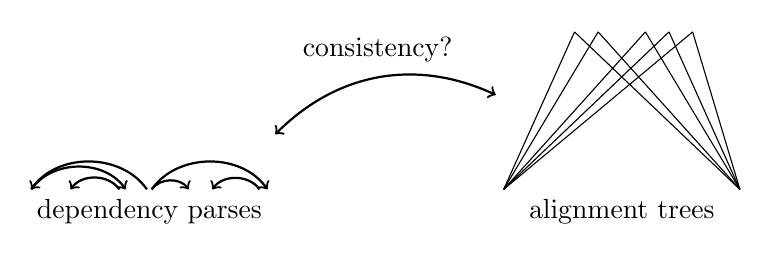
\begin{tikzpicture}

\coordinate (ss) at (1.5,0);
\node [below] at (ss) {dependency parses};

\draw[->,bend right = 55,thick] (1.47,0) to (0,0);
\draw[->,bend left = 55, thick] (1.53,0) to (3,0);
\draw[->,bend left = 55, thick] (0.0,0) to (1.2,0);
\draw[->,bend right = 55,thick] (1.12,0) to (0.5,0);
\draw[->,bend left = 55, thick] (1.53,0) to (2.0,0);
\draw[->,bend right = 55,thick] (2.9,0) to (2.3,0);

\coordinate (ts) at (7.5,0);
\node [below] at (ts) {alignment trees};

%\draw (6,0) -- (0.6,2) (9,0) -- (6.6,2);
\draw (6,0) -- (6.9,2) (9,0) -- (6.9,2);
\draw (6,0) -- (7.2,2) (9,0) -- (7.2,2);
%\draw (6,0) -- (7.5,2) (9,0) -- (7.5,2);
\draw (6,0) -- (7.8,2) (9,0) -- (7.8,2);
\draw (6,0) -- (8.1,2) (9,0) -- (8.1,2);
\draw (6,0) -- (8.4,2) (9,0) -- (8.4,2);

\coordinate (startarrow) at (3.1,0.7);
\coordinate (endarrow) at (5.9,1.2);
\node (t) at (4.4,1.5) [above]{consistency?};

\draw[<->,bend left =35, thick] (startarrow) to (endarrow);

\end{tikzpicture}
\caption{Is ther consistency between dependency parses and alignment trees?}\label{fig:depshats}
\end{figure}

\myparagraph{2. What are the reasons dependency parses are not entirely preserved during translation?}
Given previous studies, it is to be expected that dependency parses will not be entirely preserved during translation, resulting in the follow up question: what are the main bottlenecks? We will investigate what the phenomena are that cause dependency structures to change during translation.

\myparagraph{3. Can dependency grammars be used to construct a bilingual compositional grammar?}
When the direct preservation of dependency relations is assessed and the main bottlenecks are identified, a third question can be addressed, that touches on the bigger question regarding compositionality: can we use this information to construct a bilingual grammar matching translation data? As we do not develop an MT model, the answer to this last question will be rather speculative because even if a compositional grammar could be constructed, we will not test it in practice. However, we can investigate whether the answers to the previous questions can be used to create a bilingual grammar that can generalise over different sentences and alignments, has good coverage over a corpus of sentences, and is able to assign structures to sentences that are in line with their alignment.\\

In the next section, it will be discussed how this thesis intends to answer these questions. Before we, get there, we want to make a last remark about compositionality of translation, how the issue should be approached in an empirical study and how answers should be interpreted.

\myparagraph{A remark about compositionality}
It is often argued that translation cannot be treated compositionally because there are certain phenomena for which it is hard to find a compositional treatment.\footnote{A famous example that is often given is the translation of 'he swam across the river' into Spanish, where this is translated as `he crossed the river swimming', which is hard to give a compositional treatment \citep{landsbergen1989power}} In this paragraph, we want to anticipate arguments of this kind, by arguing that these phenomena are not necessarily problematic for compositional translation.

As pointed out earlier, compositionality  of translation is highly underspecified as a principle. It requires that translation of phrases should be able to be derived from the meaning of smaller parts by means of translation equivalent rules, but it is not defined how complex these rules or parts are allowed to be. When constructing a compositional grammar, phrases that cannot be translated compositionally can be included in the grammar, without that grammar formally losing the property of being compositional. We therefore want to argue that the non-compositional phenomena sitting in the corners of natural language are by themselves not arguments against the compositionality of language, and are thus not that interesting for the matter in practice. Rather, it is interesting \textit{how many} phenomena are located in this corner, and whether we can practically account for them without specifying directly for (almost) every sentence in the language what its translation is. The question `can every part of every sentence of natural language be translated compositionally' is thus not a sensible question, as the answer is: of course not. It is always possible to find odd constructions or idiomatic expressions that are hard to systematically map to another language. The important questions are: can we identify these non compositional parts in a corpus and include them in a grammar without losing the overall feeling that the grammar is compositional, and can such a grammar cover a reasonable part of natural language. Exactly these questions will be addressed in this thesis.

\section{Set-up}
\label{sec:setup}

The questions posed in the previous section will be addressed by studying alignment trees, recursive structures of translations based on word-alignments that can be interpreted as compositional translation structures. In this thesis, we will consider the subset of these structures that is maximally compositional, as defined in \cite{simaan2013hats}, that are called \textit{hierarchical} alignment trees (HATs). We will investigate the consistency of these structures with dependency parses, investigate the main causes for deviation, and propose a method for using both dependency parses and HATs to learn a compositional grammar.

In this chapter, we will discuss the main ingredients of our study. In Section \ref{sec:assumptions}, we will discuss the basis of empirical studies of translation data, and the assumptions that have to be made to conduct such research. In Section \ref{sec:comp_structures2}, we will revisit compositional translation structures. We will motivate the choice for HATs and discuss how they can be efficiently generated and represented. In Section \ref{sec:depparses}, we will briefly come back to dependency parses and provide some details of how they will be considered.


\section{Foundations of Empirical Studies}
\label{sec:assumptions}

Empirical analyses of compositionality are based on real data, that are not always perfect. When training MT models, infrequent mistakes in the data are generally not problematic, as they will receive a low probability. The same cannot be said for empirical analyses, where mistakes in the data will almost always harm the outcome. It therefore seems sensible to see empirical analysis as providing an upper- or lower bound (depending on the context) rather than an exact number. 

To appreciate empirical research, it is important to be aware of the factors that influence the results, and the necessary simplifying assumptions. In this section, we will discus these factors and assumptions, some of which may be obvious, to provide a complete picture of the foundations of empirical studies.

\subsection{Correctness of the Translation Data}

Empirical analyses based on parallel corpora with text that are each others translation rely heavily on the correctness of the data in these these corpora. As these parallel texts were not designed as data for translation models, they might not be perfectly suitable for this purpose. There are three bottlenecks.

\subsubsection{Sentence level alignment}
Aligning corpora on a sentence level is not as simple as it might seem. Texts are not always translated sentence by sentence. Short sentences may be merged or long ones broken up, and in some languages sentence delimiters do not really exist \citep[p.55]{koehn2008statistical}. However, the techniques for sentence alignment are very good, and as the languages we are considering \textit{do} have clear sentence delimiters it seems very reasonable to assume that the sentences in the corpora are correctly aligned.

\subsubsection{Correctness of translation}
The translations of the sentences are produced by humans, who sometimes make mistakes. To use the corpora, we have to assume that the aligned sentences are good translations of each other.

\subsubsection{Translation is literal}
One English sentence often has many translations in another language, as similar meanings can be expressed in multiple ways.\footnote{In fact, considering only one target translation can also be seen as a simplification made in empirical research, and in MT in general.} For instance `jeg giver dig blomster' is a good Danish translation of `I give you flowers', but so is `jeg giver blomster til dig' (and this is not even an example in which many things are rephrased). Especially when one text is not a direct translation of the other text, but the two are, for instance, just separate reports of the same event, it might happen that sentences do have the same meaning, but differ in form. In our analysis, we will assume that at least the vast majority of the translations in the corpora are rather literal.
 
\subsection{Correctness of Word Alignments}

In empirical analyses as well as MT-models, word-alignments are of crucial importance, as they are used to establish translational correspondences. Unfortunately, automatic alignments are not always as good as we want them to be \citep[see][for concrete numbers]{och2000improved}. MT-models generally do not suffer much from this fact, because the number of wrong alignment links is dwarfed by the number that is correct. For empirical research, false alignment links are quite problematic, as even one wrong link can have a huge effect on the space of possible translation trees. An option is to use one of the few manually aligned corpora, but given their small size they are not suitable to draw conclusions about larger parts of language.

\subsection{Correctness of Dependency Parses}

To determine the dependency structures of the sentences in the corpus, an efficient fully-automated dependency parser is needed.  For English, high quality dependency parses are available \citep{cer2010parsing}, but the parses they produce are not perfect, which can be problematic for an empirical analysis.



\section{Translation Structures}
\label{sec:comp_structures2}

HATs constitute a very important part of our thesis, as they represent our interpretation of compositionality. In this section we will motivate the choice for HATs, by explicating their advantageous properties. Furthermore, we will suggest a method for representing and generating them, which is given their huge number not trivially time or space efficient.

\subsection{HATs}

Although we use the term HATs to refer to them, the translation structures that are considered in this paper differ in one aspect from how they were originally defined in \citep{simaan2013hats}. \citeauthor{simaan2013hats} augmented the nodes of the HATs with operators that describe how their children should be permuted to obtain the corresponding target side HAT. We will not consider these operators in this thesis. Ultimately, the operators are necessary to fully describe the translation, as without them the target side structure of a sentence cannot be retrieved from the source side structure. However, in this thesis we take a step back, by solely considering if the skeletons of the purely bilingually motivated HATs can describe the source language in a monolingual fashion. We will thus not pay any attention to the target side languages, but only consider the structural restrictions the translation into target language sentences places on the structure of the source sentences. If it is possible to find a monolingual system for the source language that corresponds with these bilingual constraints, a next step is of course to take into account the operators and reordering phenomena to consider the target side structures.

\subsection{Motivation for using HATs}

Recall that a HAT is a maximally compositional alignment tree, which means it is characterised by the following set of properties:\begin{enumerate}
\item A HAT is a projective tree whose leaf nodes form a sentence.
\item A HAT describes a compositional translation of the sentence constituted by its leaf nodes.
\item All non-terminal nodes of a HAT dominate a sequence that is translation admissible according to the alignment of the sentence, while sibling terminal nodes together constitute a translation admissible sequence.
\item A node in a HAT can have both non-terminal and terminal child nodes at the same time.
\item All nodes in a HAT expand into a minimal number of children.
\end{enumerate}

\noindent A HAT is thus an alignment tree that describes a maximally compositional translation of a sentence. 

The property of being maximally compositional gives HATs several attractive properties, which we will discuss in this subsection.

\subsubsection{Computational}
There is a clear computational advantage to considering only minimally branching trees. Not only does it significantly reduces the space of trees to be considered - the example sentence previously used in Section \ref{sec:comp_structures} for explaining alignment trees\footnote{Sentence pair: (`My dog also likes eating sausages', `Mijn hond houdt ook van worstjes eten')\\Set-permutation: $\langle \{0\}, \{1\}, \{3\}, \{2,4\}, \{6\}, \{5\}\rangle$. } has 44 alignment trees, but only 5 of them are minimally branching - it also simplifies parsing, as the lower-rank rules that can be extracted from minimally branching trees can be more efficiently treated by parsing algorithms.

\subsubsection{Theoretical}

Of course, such computational considerations are less important for an empirical analysis (although even for empirical analysis computational requirements should match the reality). However, maximal compositionality also has some attractive properties besides the compositional ones, which we will explicate in the following paragraphs.

\paragraph{Compositionality} Considering only minimally branching trees secures that the system we are studying is in fact compositional. The set of all alignment trees contains many flat trees, that can strictly speaking be seen as compositional (as compositionality is highly underspecified in this respect), but do not capture the recursive and systematic nature of language. A compostional system containing a separate rule for almost every sentence that specifies how its meaning can be derived from \textit{all of its words} does certainly not correspond with human intuitions about compositionality, not to mention the fact that such a system should have an infinite number of rules to cover the entire language. Considering only minimally branching trees solves this problem.

\paragraph{Generalisation} Considering only expansions that are maximally compositional maximises the chance that generalisation to new data is possible: a rule that specifies how a type of argument can be combined with a type of predicate is more useful than a rule specifying how the argument `I' can be combined with the predicate `like'. Minimum depth expansions are more probable to be applicable in new situations. 

Figure \ref{fig:nepas} shows how French negation, often mentioned as problematic for structure based systems, is accounted for with a HAT skeleton. The translation tree shows that `I dont like' is the translation of `Je n'aime pas', but also contains the information that `don't' is phrasally translated as `ne ... pas'. Removing the negation in the English sentence results in the grammatical English sentence `I like cars', removing its translation equivalent in the French sentence in its (almost) grammatical `Je aime les voitures'. If `I don't like' was generated in one rule, this generalisation would not have been possible.

\begin{figure}[!ht]
\centering
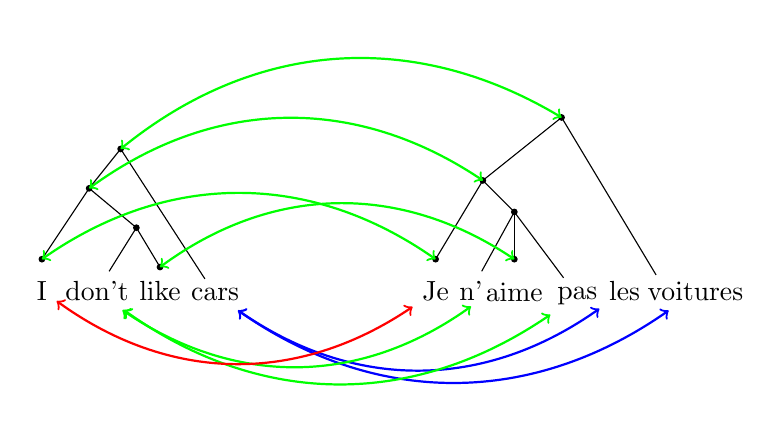
\begin{tikzpicture}
\draw node (I) at (0,0) {I};
\draw node (dont) at (0.7,0) {don't};
\draw node (like) at (1.5,0) {like};
\draw node (cars) at (2.2,-0.05) {cars};

\draw node (Je) at (5.0,0) {Je};
\draw node (n) at (5.45,0) {n'};
\draw node (aime) at (6.0,-0.02) {aime};
\draw node (pas) at (6.8,-0.07) {pas};
\draw node (les) at (7.4,0) {les};
\draw node (voitures) at (8.3,-0.01) {voitures};

\coordinate (Je_) at (5.0,0.4);
\coordinate (like_) at (1.5,0.3);
\coordinate (I_) at (0,0.4);
\coordinate (aime_) at (6.0,0.4);
\coordinate (naimepas) at (6.0,1);
\coordinate (dontlike) at (1.2,0.8);
\coordinate (Idontlike) at (0.6,1.3);
\coordinate (Jenaimepas) at (5.6,1.4);
\coordinate (lesvoitures) at (7.8,0.2);
\coordinate (all) at (1,1.8);
\coordinate (tout) at (6.6,2.2);
\coordinate (n_) at (5.45,-0.2);

\foreach \coordinate in {dontlike, like_, I_, Je_, aime_, Idontlike, all, tout, Jenaimepas, naimepas}
	\filldraw (\coordinate) circle (0.035);

\foreach \from/\to in {naimepas/aime_, naimepas/n, naimepas/pas, dontlike/like_, dontlike/dont, Idontlike/I_, Idontlike/dontlike, all/Idontlike, all/cars, Jenaimepas/Je_, Jenaimepas/naimepas, tout/Jenaimepas, tout/lesvoitures}
	\draw (\from) -- (\to);

\foreach \from/\to in {cars/voitures, cars/les}
	\draw[<->, bend left = -35, thick, blue] (\from) to (\to);

\foreach \from/\to in {dont/n_, dont/pas, tout/all, Jenaimepas/Idontlike, aime_/like_, Je_/I_}
	\draw[<->, bend left = -35, thick, green] (\from) to (\to);

\draw[<->, bend left = -35, thick, red] (I) to (Je);

\end{tikzpicture}
\caption{Translation of negation, French-English}\label{fig:nepas}
\end{figure} 

\paragraph{Preservation of structure of phrasal translations}

An advantage that overlaps with the two previously mentioned advantages, but is worth noting nonetheless, is the fact that structure of phrasally translated sequences is preserved, if possible. As the rest of the tree, sequences of words will be translated as a phrase only if they do not have a deeper structure according to the translation data. In many phrase-based translation systems, including the successful hierarchical phrase based system proposed by \cite{chiang2007hierarchical}, the underlying structure of sequences that are translated phrasally gets lost in the process,\footnote{This simplification is mostly made for efficiency reasons.} whereby the system misses an opportunity to detect a pattern. HATs fully exploit recursiveness, also in idiomatic and phrasal translations. We will revisit an example containing syntactic divergence to illustrate how a structural treatment of phrasal translation is helpful.

In Russian, `X has Y' is (somewhat communistically) translated as `with X is Y', the object in English is thus the subject in Russian. Figure \ref{fig:russian1} shows how this is dealt with in a translation structure. Due to the structural treatment of the phrasal translation, this translation tree is easily extendible to longer sentences with the same construction. By expanding the non-terminal nodes it can also capture sentences like `the girl with the long blond hair has a very old car with broken windows'.

\begin{figure}[!ht]
\centering

\begin{tikzpicture}

\draw node (the) at (0,0.02) {The};
\draw node (girl) at (0.75,0) {girl};
\draw node (has) at (1.4,0.04) {has};
\draw node (a) at (1.9,0) {a};
\draw node (car) at (2.4,0) {car};
\draw node (y) at (4,0) {\textcyr{u}};
\draw node (girlr) at (4.9,-0.02) {\textcyr{devuxki}};
\draw node (is) at (6.1,0.02) {\textcyr{est\char126}};
\draw node (carr) at (7.5,0.04) {\textcyr{avtomobil\char126}};

\coordinate (thegirl) at (0.4,0.6);
\coordinate (acar) at (2.1,0.6);
\coordinate (thegirlhas) at (0.8,1);
\coordinate (all) at (1.4,1.5);
\coordinate (carr_) at (7.5, 0.3);
\coordinate (girlr_) at (4.9,0.3);
\coordinate (girlhas) at (4.9,0.8);
\coordinate (allr) at (5.9, 1.2);


\foreach \coordinate in {thegirl, acar, thegirlhas,all,carr_, girlr_, girlhas, allr}
	\filldraw (\coordinate) circle (0.035);

\foreach \from/\to in {thegirl/girl, thegirl/the, acar/a, acar/car, thegirlhas/thegirl, thegirlhas/has, all/thegirlhas, all/acar, girlhas/girlr_, girlhas/y, girlhas/is, allr/girlhas, allr/carr_}
	\draw (\from) -- (\to);

\foreach \from/\to in {the/girlr, girl/girlr}
	\draw[<->, bend left = -35, thick, blue] (\from) to (\to);

\foreach \from/\to in {has/y, has/is, allr/all, girlhas/thegirlhas, carr_/acar, girlr_/thegirl}
	\draw[<->, bend left = -35, thick, green] (\from) to (\to);

\foreach \from/\to in {a/carr, car/carr}
	\draw[<->, bend left = -35, thick, red] (\from) to (\to);

\end{tikzpicture}
\caption{A graphical representation of the translation of possession from Russian to English.}\label{fig:russian1}
\end{figure}


\subsubsection{Critical Note}

Intuitively, maximal compositionality sometimes seems somewhat strict. When constructing a sentence that has an predicate with two arguments, it is linguistically not always desirable to assume that the predicate is combined with the arguments one by one. In translation, this issue is enhanced by the fact that arguments of a predicate may not be in the same order for different languages. A HAT describing a translation in which this happens is forced to combine the arguments with each other before combining them with the predicate, which may sometimes seem counterintuitive.


\subsection{Representational Aims}

To study HATs, we need to be able to generate HATs for every sentence, and store them in a suitable fashion. Generating and storing all trees separately would be both time and space consuming, and would impede a flexible search through them. Hence, a suitable representation of the set of HATs is required. This representation should be easy to search, preferably memory efficient, flexible to abstract information from and easy to combine and compare with other representations of sets of HATs.

The original HAT paper also presented an implementation for generating and storing HATs. The HAT-forests of sentences were represented as a compact chart. Unfortunately, this implementation could not be used for the purpose of this paper. The chart representation was not easily accessible as an object, and modifying the program that generated it to obtain the desired properties did not seem within reach. Furthermore, unaligned words were completely ignored. In some cases, this might be a reasonable simplification, but for empirical analysis this is not desirable.

For this thesis, we aimed to find a new representation of a set of HATs that has both the efficient properties of the current implementation, but is more flexible and accessible, and easy to use for other purposes than precisely the one of this paper. In this subsection, we will explain how we will represent and generate HATs. Documentation of the complete implementation can be found in Appendix \ref{appendix:implementation}. To make the representation easily accessable for people unfamiliar with the code, we have implemented several demo's to illustrate the use and possibilities of the HATs.


\subsection{Representation}

We have represented a set of HATs implicitly by a CFG that describes for every (translation admissible) span of the sentence how it is allowed to expand. By default, the nodes are labelled with the span they dominate, but labels for spans can be provided. Figure \ref{fig:grammar} provides an example.

HATS represented as context free grammars are easy to wield. As the labels are unique, the HAT CFG can be easily unpacked into all HATs for a sentence (which we will never do), but can also recursively be investigated. E.g., the number of HATs can be determined efficiently in a top-down fashion, and parsing with the HATgrammar can provide information about several of its properties.

\begin{figure}\begin{framed}
\small{
\begin{tabular}{llllll}
(0-6] $\rightarrow$ (0-1]  (1-6] && (4-6] $\rightarrow$ (4-5]  (5-6] && (0-1] $\rightarrow$ My\\
(0-6] $\rightarrow$ (0-2]  (2-6] && (0-4] $\rightarrow$ (0-1]  (1-4] && (1-2] $\rightarrow$ dog\\
(0-6] $\rightarrow$ (0-4]  (4-6] && (0-4] $\rightarrow$ (0-2]  (2-4] && (2-3] $\rightarrow$ also\\
(1-6] $\rightarrow$ (1-4]  (4-6] && (1-4] $\rightarrow$ (1-2]  (2-4] && (4-5] $\rightarrow$ eating\\
(1-6] $\rightarrow$ (1-2]  (2-6] && (0-2] $\rightarrow$ (0-1]  (1-2] && (5-6] $\rightarrow$ sausages\\
(2-6] $\rightarrow$ (2-4]  (4-6] && (2-4] $\rightarrow$ (2-3] likes\\
\end{tabular}
\caption{The grammar generating the translation tree forest for the sentence
`My dog also likes eating sausages', with set-permutation $\langle _0\{0\}_1,~ _1\{1\}_2,~ _2\{3\}_3,~ _3\{2,4\}_4, ~_4\{6\}_5,~ _5\{5\}_6\rangle$ would be (the subscripts indicating the span annotation, which is left exclusive and right inclusive)}\label{fig:grammar}
}
\end{framed}
\end{figure}

\subsection{Generation}
To generate the HAT forest for an alignment, it suffices to find the minimal segmentations for all contiguous translation admissible subsequences of the alignment. We generated the set of contiguous translation admissible subsequences (i.e., the source sides of all phrase pairs) with the shift-reduce algorithm presented in \cite{zhang2008extracting}. Some small adaptations were necessary to generate the full set of phrase pairs, rather than only the `tight' subset, in which unaligned words at the boundaries were not included. To find the minimal segmentations of all phrases we used \citepos{dijkstra1959note} shortest path algorithm (Algorithm \ref{alg:shortest paths}), that we adapted to search for \textit{all} shortest paths rather than just one, and to incorporate the information that, given the direction of the edges, only searching in nodes with a larger value could actually lead to a shortest path, which made the search more efficient. Details are provided in Algorithm \ref{alg:shortest paths}. For memory efficiency, all paths were stored in a linked list with path points that were shared among different paths.

\begin{algorithm}
\caption{Shortest Paths}\label{alg:shortest paths}
\begin{algorithmic}
\STATE \textbf{Input:} A graph $G = (V,E)$ describing an alignment and two vertices $i$ and $j$ for which $(i,j)\in E$ is true.
\STATE \textbf{Output:} All non-trivial shortest paths from $i$ to $j$
\STATE \textit{\#Initialization}
\STATE visited = $\emptyset$, depth = $0$, paths = $\{j\}$
\STATE $\forall n\in\mathbb{N}:$ reachable(n) = $\emptyset$; reachable($0$) = $\{j\}$
\STATE depth\_finished = False
\STATE \textit{\# Start backwards search through graph}
\WHILE{not depth\_finished or $i\notin$ visited}
	\WHILE{reachable(depth) $\neq\emptyset$}
		\STATE depth\_finished $\leftarrow$ False
		\STATE current\_node $\leftarrow N$ an arbitrary element $v$ from reachable(depth)
		\STATE reachable(depth) $\leftarrow$ reachable(depth) $-$ $\{$current\_node$\}$
		\FOR{ ($l$,current\_node) $\in E$}
			\IF{$l\notin $visited $\cup$ reachable(depth) \AND depth $\neq 0$}
				\STATE reachable(depth+1) $\leftarrow$ reachable(depth+1) $\cup$ $\{l\}$
				\FOR{path (current\_node,\ldots, $j) \in$ paths}
					\STATE path $\leftarrow$ ($l$,current\_node,\ldots, $j)$
				\ENDFOR
			\ENDIF
		\STATE visited $\leftarrow$ visited $\cup$ $\{l\}$
		\ENDFOR
	\STATE depth\_finished $\leftarrow$ True
	\STATE depth $\leftarrow$ depth+1
	\ENDWHILE
\ENDWHILE
\STATE \textbf{Return} paths
\end{algorithmic}
\end{algorithm}


\section{Dependency parses}
\label{sec:depparses}

As we have elaborately discussed dependency parses earlier in Section \ref{sec:dep_parses}, we will only briefly revisit them in this section, and discuss how we obtain them.

Several assumptions can be made about dependency parses. In this thesis it is assumed, following common practice, that a dependency structure satisfies the following two conditions:\begin{enumerate}
\item When seen as a relation, $D$ constitutes a single-headed acyclic connected graph in which the words in $s$ are the nodes. (tree-constraint)
\item When the words are placed in the original order, the branches of the dependency tree do not cross. (projectivity)
\end{enumerate}

\subsection{Representation}

We will represent a dependency parse of a sentence $s = w_0\cdots w_n$ as a set of relations $D = \{(i,j)|$ there is a dependency arrow from word $w_i$ to word $w_j \}$. 

Formally, dependency grammars are not interpreted as compositional grammars, as they do not postulate the existence of non-terminal syntactic categories. That is, dependency parses describe predicate-argument relations between \textit{words} and not between larger parts, and do thus not explicitly specify the recursive structure of a sentence. However, dependency graphs do give rise to a hierarchical structure, that specifies from which smaller parts the sentence was composed. For instance, the dependency graph depicted in Figure \ref{fig:deptree} tells us that `likes' is the head word of the sentence, and that the sentence is composed of 4 parts: the head `likes', its modifier `also', its noun subject whose head is `dog' and the open clausal complement whose head is `eating'. The complement and subject are further divisible in `My' and `dog', and `eating' and `sausage', respectively. As the tree is projective, all parts are continuous. Also the graph in Figure \ref{fig:depgraph} we saw earlier prescribes an hierarchical structure: it is composed of the subject `I', the headword `know', and the phrase headed by `liet', that is in its turn built up from its head `liet', `dat', `hij' and the discontinous phrase `me winnen'. Such an hierarchical structure cannot be captured by a phrase structure grammar.

\begin{figure}[!h]\label{fig:deptree1}
\centering
\begin{dependency}[theme=simple]%[hide label]
\begin{deptext}[column sep=.5cm, row sep=.1ex]
%PRP\$ \& NN \& RB \&[.5cm] VBZ \& VBG \& NN \\
My \& dog \& also \& likes \& eating \& sausage \\
\end{deptext}
\deproot{4}{}
\depedge{2}{1}{poss}
\depedge{4}{2}{nsubj}
\depedge{4}{3}{xvmod}
\depedge{4}{5}{xcomp}
\depedge{5}{6}{dobj}
\end{dependency}
\caption{Stanford Dependency Tree}\label{fig:deptree}
\end{figure}

\subsection{Generation}

To assign dependency structures to sentences, we used the Stanford Dependency Parser, that can be downloaded from their website, as well as used online  \citep{de2006generating}. The parser provides 5 variants of a typed dependency representation, of which the most basic one corresponds to the earlier imposed conditions on dependency structures \citep{de2008stanford}. A picture of a dependency parse that was generated by the parser is depicted in Figure \ref{fig:deptree}.

Unfortunately, the Stanford dependency parser used does not cover all tokens of the input sentences, as dependency relations between words and punctuation are not present in the Stanford Dependency Representation. The resulting dependency trees do thus not always cover the entire sentence.

\section{Summary}
\label{sec:summary4}

In this chapter we have presented the basis for the original research conducted for this paper. At the start of this chapter we have stated the aims of this research, and provided a short summary of the background we presented in earlier chapters. We formulated three questions\begin{enumerate}
\item Are dependency structures universal for languages?
\item What are the reasons that dependency parses are not entirely preserved during translation?
\item Can dependency grammars be used to construct a bilingual compositional grammar?
\end{enumerate}

We have listed the main assumptions that we made in our empirical investigation of the three questions presented, and we have revisited the two main ingredients of this investigation: HATs and dependency parses.
%\bibliography{thesisDH}
%\end{document}